\documentclass{article}

% ============================================================
% NeurIPS 2026 style, PREPRINT option so author names are shown
% (course deliverable, not an anonymous submission).
% ============================================================
\usepackage[preprint]{neurips_2026}

\usepackage[utf8]{inputenc}
\usepackage[T1]{fontenc}
\usepackage{hyperref}
\usepackage{url}
\usepackage{booktabs}
\usepackage{amsfonts}
\usepackage{amsmath}
\usepackage{nicefrac}
\usepackage{microtype}
\usepackage{xcolor}
\usepackage{graphicx}
\usepackage{pgfplots}
\pgfplotsset{compat=1.17}
\usepackage{listings}   % code snippets in appendix C
\lstset{basicstyle=\ttfamily\small, breaklines=true, frame=single,
        columns=fullflexible, showstringspaces=false}

\newcommand{\flag}{\textcolor{red}{\textbf{[?]}}}
\usepackage{siunitx}
% ---- Per-section contribution tags. Set to \relax to hide. ----
% \newcommand{\contrib}[1]{\textcolor{gray}{\small\textit{[#1]}}}
\newcommand{\contrib}[1]{}

% ============================================================
% TITLE  -- placeholder; lock to the ACTUAL finding once results final.
% ============================================================
\title{Behavioral Conditioning of Video World-Model Predictors\\
for Egocentric Action Anticipation}

% ============================================================
% AUTHORS  (course project -- real names, real emails)
% ============================================================
\author{%
  Seyyed Parsa Sharifi \\
  University of Rostock \\
  \texttt{seyyed.sharifi@uni-rostock.de} \\
  \And
  Erfan Yekehzare \\
  University of Rostock \\
  \texttt{erfan.yekehzare@uni-rostock.de} \\
}

\begin{document}

\maketitle

% ---- GITHUB LINK (Ashwin req 3: link must appear in the report) ----
\begin{center}
\fbox{\parbox{0.9\linewidth}{\centering
\textbf{Code:} \url{https://github.com/EgocentricPerceptions/CV4Egocentric_Semantic_Intention_Prediction}
\quad$\bullet$\quad
Project: EgoProject 2026 (Univ.\ Rostock $\times$ UBB Cluj)
}}
\end{center}

% ============================================================
% ABSTRACT  -- humanized pass (2026-08-13). Varied cadence, fewer em-dashes.
% ============================================================
\begin{abstract}
Egocentric action anticipation depends on reading preparatory cues before an
action becomes visible. Human behavioral signals are an obvious place to look for
those cues: gaze tends to precede manipulation, and the hands are what turn
intention into action. We ask whether conditioning a frozen V-JEPA~2 predictor on
gaze and hand pose improves short-horizon anticipation on EPIC-KITCHENS-100. It
does not, and the aim of this paper is to say why with some precision. We turn the
existing peer-token conditioning pathway into a bit-exact control, add a guard
against three failure modes that can each counterfeit a null, and run five diagnostics against the frozen predictor and the behavioral signal
itself. We then repeat the predictor's own training with the signal ablated,
which separates the value of the information from the cost of withholding an
input the model expects. The results agree: the signal reaches the predictor's
output, the predictor is indifferent to its content, a predictor that never saw
the signal matches one trained with it, and on its own the signal beats a class
prior by under two points. We therefore retired a stronger, GazeQwen-informed pathway at the
design stage rather than after paying to build it. One effect does survive.
Behavioral signals favour verbs, which encode motion, while vision favours nouns,
which encode object identity, and the same split organises the two strongest
published systems on this benchmark. But once the vision comparator is fitted
fairly, the effect holds only in direction and never rises above the verb prior,
and the constraint that bounds it is single-participant sample size rather than
any floor in the probe's dynamic range. We read the null as evidence that
feeding these signals in at the input is the wrong way to use them, and argue for
supervising the representation with behavioral signals toward goal-level targets
instead. The anticipation results here are bounded to one participant at a
one-to-two-second horizon; the training-side ablations that carry the null are
cross-participant.
\end{abstract}

% ============================================================
% 1. INTRODUCTION -- humanized pass. Break symmetric signposting,
% vary constructions, keep the three contribution bullets (they work).
% ============================================================
\section{Introduction}

Anticipating what a person will do next from egocentric video is hard for a
structural reason: the most discriminative evidence, the action itself, has not
happened yet. The model has to work from preparatory cues instead. Human
behavioral signals are a natural candidate for those cues. Gaze leads
manipulation by something like half a second to a second, and the hands are the
effector that carries out intention, so conditioning a predictive model on gaze
and hand pose ought to help it anticipate.

V-JEPA~2 \citep{assran2025vjepa2} makes that idea testable. It learns a frozen
encoder and a latent predictor by predicting masked spatiotemporal features, and
its action-conditioned variant conditions the predictor on robot actions. We ask
whether the same predictor can be conditioned on \emph{human} signals instead,
gaze and hand pose from egocentric recordings, and whether that improves action
anticipation on EPIC-KITCHENS-100 (EK100) \citep{damen2022ek100}. Earlier phases
of the project had already returned a stubborn null at the two-second horizon,
and a control family had suggested that what looked like an effect of
conditioning was mostly an effect of feeding the model more tokens. That left one
question unanswered, with two answers that point in opposite directions. Perhaps
the injection pathway is too weak to expose whatever the signal carries; perhaps
the signal simply does not carry action-relevant information at this horizon. The
first answer argues for a stronger architecture. The second argues for giving up
on input-level conditioning altogether.

This paper sets out to decide between those two rather than assume either. The
contribution is diagnostic, and we state it plainly, null included:
\begin{itemize}
  \item We make the existing peer-token pathway a bit-exact control and guard
        against three silent-failure modes that can each fake a null, so that the
        null we report is a property of the signal and the pathway, not an
        artifact of the evaluation code (\S\ref{subsec:method-weak}).
  \item We run five diagnostics directly against the frozen predictor and the
        behavioral signal. They tell a consistent story: the signal reaches the output, the predictor
        ignores its content, and on its own the signal anticipates the next
        action barely above a class prior (\S\ref{subsec:diagnostics}). Varying
        the training rather than the input confirms it: a predictor whose
        training never included the signal matches one trained with it
        (\S\ref{subsec:training-ablation}). That evidence let us retire a stronger,
        GazeQwen-informed \citep{pham2026gazeqwen} pathway at the design stage
        instead of after building it (\S\ref{subsec:b4}).
  \item We isolate the one effect that does survive, a motion-specific advantage
        of behavioral signals on verbs over vision, and show that under a fair
        comparator it holds only in direction, never above the verb prior, and
        that the real constraint is single-participant sample size, not a floor
        in dynamic range (\S\ref{subsec:dissociation}--\ref{subsec:ddn}).
\end{itemize}
The result is a null we can explain rather than one we merely report, and the
explanation points past input-level conditioning toward representation-level
supervision of behavioral signals (\S\ref{sec:conclusion}). We keep every anticipation claim bounded to one participant at roughly one to two
seconds; the training-side ablations reach across participants, and we flag which
is which where it matters.
% ============================================================
% 2. BACKGROUND / RELATED WORK
% Erfan owns 2.1 (JEPA/VL-JEPA) -- sized stub.
% Parsa: 2.2 (gaze-conditioning) + 2.3 (project origin, from EARLY_WORK_SUMMARY.md).
% 2.3 REWRITTEN 2026-08-13: real origin = 5-phase plan -> confounded 2.81/4.27
% pilot. Context-selection thread demoted to one sentence.
% ============================================================
\section{Background and related work}

% ------------------------------------------------------------
\subsection{Joint-embedding predictive architectures for video}
\label{subsec:bg-jepa}
% -----------------------------------------------------------------------------
% ERFAN: the JEPA lineage that sets up our method. Suggested coverage:
%   - I-JEPA (image, latent prediction vs pixel reconstruction) \citep{assran2023ijepa}
%   - V-JEPA / V-JEPA 2 / 2.1 (video feature prediction; frozen encoder+predictor)
%     \citep{bardes2024vjepa, assran2025vjepa2, murlabadia2026vjepa21}
%   - DINO-WM (world models on frozen features) \citep{zhou2024dinowm}
%   - VL-JEPA / language-aligned latent prediction -- YOUR section, tie to horizon.
%   - EgoAgent (joint predictive agent model, egocentric) \citep{chen2025egoagent} -- adjacent framing.
%   - the AC (action-conditioned) predictor as the thing we re-purpose for HUMAN signals.
% Keep it tight; \S\ref{subsec:method-setup} carries the setup detail.
% -----------------------------------------------------------------------------
\paragraph{Latent prediction.}
The lineage this work builds on replaces pixel reconstruction with prediction in
representation space. I-JEPA~\citep{assran2023ijepa} established the pattern for
images: from a context block, predict the \emph{embeddings} of masked target
blocks rather than their pixels, so the objective is never forced to model detail
that carries no semantic content. V-JEPA~\citep{bardes2024vjepa} carried the idea
to video, and V-JEPA~2~\citep{assran2025vjepa2} scaled it. Its three components
fix the vocabulary we use throughout: a student encoder that sees the visible
patches, a teacher encoder updated by exponential moving average that supplies
target embeddings under a stop-gradient, and a \emph{predictor} that maps the
student's context embeddings plus positional queries for the masked positions
onto what the teacher would emit there. The entire training signal is a distance
between predicted and target latents; nothing is ever rendered to pixels.
V-JEPA~2.1~\citep{murlabadia2026vjepa21} revises the recipe toward denser
features, and is the backbone of both frozen-probe systems that currently lead
EK100 anticipation (\S\ref{subsec:bg-gaze}).

\paragraph{Frozen features as a world model.}
The encoder/predictor split matters because the two can be used separately.
DINO-WM~\citep{zhou2024dinowm} builds a world model on top of frozen visual
features and plans by optimising action sequences against predicted future
latents, which is evidence that a frozen representation plus a learned latent
predictor is already enough to support prediction-based control. Our protocol
rests on the same assumption in a weaker form: we never fine-tune the
representation, and read anticipation out of it with a deliberately small probe
(\S\ref{subsec:method-setup}).

\paragraph{The action-conditioned predictor, and what we re-purpose.}
V-JEPA~2 also ships an action-conditioned variant (V-JEPA~2-AC), in which the
predictor is additionally conditioned on robot end-effector action and state,
each encoded to a token and concatenated as a peer alongside the visual tokens
\emph{inside} the predictor. That token layout is precisely the interface this
paper re-purposes: we substitute human gaze and hand pose for the robot's action
and state and change nothing else about the pathway
(\S\ref{subsec:method-weak}). EgoAgent~\citep{chen2025egoagent} makes an adjacent
move in the egocentric setting, learning representation, prediction and action
jointly rather than treating them as separate stages.

\paragraph{Language-aligned latent prediction.}
A final branch of the lineage moves the \emph{target} of latent prediction from
appearance toward meaning. VL-JEPA~\citep{vljepa2025} predicts the embedding of
an answer rather than generating it token by token, so that two paraphrases of
the same content land near each other instead of being orthogonal in token space,
and the semantics are available without waiting for a decode. Its relevance here
is directional rather than architectural: it demonstrates that the JEPA objective
survives a change of target, which is exactly the move our own results argue for
in place of input-level conditioning --- supervising the representation toward
goal- or intention-level targets rather than concatenating a signal at the input
(\S\ref{sec:conclusion}).

% ------------------------------------------------------------
\subsection{Conditioning prediction on behavioral signals}
\label{subsec:bg-gaze}

A parallel line of work asks how gaze and body signals should enter a predictive
model, and it divides usefully by where the signal is injected. At one end sit
input concatenation methods, the peer-token approach this paper diagnoses. At the
other, signals supervise the representation during training and are discarded at
inference. GABRIL \citep{banayeeanzade2025gabril} regularises an
imitation-learning representation toward human gaze to mitigate causal confusion;
the gaze-regularised vision-language models of \citet{pani2026gazereg} align model
attention to gaze via a regularisation term and report improved future-event
prediction without gaze at inference; and \citet{royfernando2022abstractgoal}
model an abstract goal distribution and a goal-consistency objective for
next-action selection. A related line conditions anticipation explicitly on
intention or goal: the intention-conditioned VAE of \citet{mascaro2023icvae}, the
goal-conditioning isolated by AntGPT \citep{zhao2024antgpt}, the intention-guided
cognitive reasoning of \citet{chu2026intention}, and the gaze-guided,
intention-conditioned graph network of \citet{ozdel2024gazegnn} all report that an
intention or goal signal improves long-term anticipation, a pattern our own
results echo in pointing away from input-level conditioning and toward goal-level
targets. Anticipating the behavioral signal itself has also been studied
directly, as in the audio-visual egocentric gaze anticipation of
\citet{lai2024listentolook}. Between these, GazeQwen \citep{pham2026gazeqwen}
modulates a frozen video-language model with gaze through a lightweight resampler
that adds residuals at decoder layers, and argues that the obstacle is a missing
learned pathway from gaze into the model's internal representations rather than a
deficiency of the signal. That framing organises our own investigation: we adapt
GazeQwen's mechanisms as the template for a stronger pathway, but test whether
such a pathway could help before building it (\S\ref{subsec:method-strong}).

On the benchmark itself, the two strongest published EK100 anticipation systems
are both frozen-V-JEPA-2.1 attentive probes \citep{chu2026jfaa, wang2026tapjepa}.
Neither conditions on behavioral signals, yet both split their probes into
separate verb and noun heads on the reasoning that verbs track motion and nouns
track object appearance, a split that reappears in our own results
(\S\ref{subsec:dissociation}). They mark the vision-only ceiling of the
frozen-probe regime, and they leave our question, whether behavioral conditioning
adds anything on top, untested.

% ------------------------------------------------------------
\subsection{Project origin}
\label{subsec:bg-origin}

This study grew out of an earlier attempt to carry V-JEPA~2's action-conditioned
predictor from robot manipulation to egocentric human video, replacing the
robot's end-effector action and state tokens with human gaze and hand-pose
tokens. (An even earlier exploratory step had used gaze only to bias
\emph{context selection} for masked reconstruction, and found no benefit at high
coverage; it did not lead anywhere and we mention it only for completeness.) The
conditioning effort was organised as a five-stage plan: reproduce the published
EK100 anticipation baseline, train an own probe to own that baseline, map the
action-conditioned predictor's architecture, post-train the predictor on HD-EPIC
with gaze and hand tokens, and re-probe on EK100 to measure the change.

The plan did not survive contact with a deadline, and the first behavioral
comparison was confounded by design. The from-scratch behavioral predictor
trained on HD-EPIC was a ViT-L model, but the only fine-tuned
behavioral checkpoint available in time was the ViT-G model from the project's
own conditioning track, trained separately and with a differently-shaped
(three-dimensional) gaze input. Rather than wait, the comparison
was run across encoders, knowingly unfairly: a ViT-L vision baseline reached
$4.27\%$ action R@5 on EK100 while the ViT-G behavioral arm reached $2.81\%$, with
the behavioral arm also behind on verb and noun recall, feature silhouette, and
nearest-neighbour retrieval. Both sides were trained for a single probe epoch and
were underfit. The number is therefore directional only, and we treat it as a
confounded pilot rather than a result: the encoders differ, the predictors come
from different training runs, and gaze is masked at EK100 evaluation. What the
pilot did establish was the question this paper takes up. Behavioral conditioning
had not helped, and it was not yet clear whether the fault lay with the injection
pathway, the confounds, or the signal itself. The controlled study that follows
was built to separate those explanations.
% NOTE: origin sourced from EARLY_WORK_SUMMARY.md (reconstructed from ocean-cluster
% session transcripts + live CLAUDE.md/eval_report.md). 4.27 = Phase 2 ViT-L
% baseline; 2.81 = Phase 5 ViT-G behavioral (colleague checkpoint). Deliberately
% confounded, directional only -- do NOT upgrade to a headline result.
% ============================================================
% 3. METHOD
% ============================================================
% DRAFT v0.1 (2026-08-13). Solid draft, NOT final. Seams marked "FLAG:".
% DISCIPLINE: STRONG pathway is DESIGNED, NOT BUILT. Never say implemented/ran.
% Ashwin quote (22 Jul) woven in; accuracy guard applied (Parsa proposed the
% (b)-reading, Ashwin endorsed -- do NOT imply Ashwin proposed it end-to-end).
% ============================================================
\section{Method}
\contrib{lead: Parsa}

Our method is a frozen-representation probe of whether egocentric behavioral
signals carry action-anticipatory content, together with a controlled pathway
by which those signals are injected into the predictor. We first describe the
frozen-probe setup and evaluation protocol (\S\ref{subsec:method-setup}), then
the two conditioning pathways: a weak one that is built and verified, and a
stronger one that is deliberately specified but left unimplemented
(\S\ref{subsec:method-weak}--\ref{subsec:method-strong}). Last comes the
direct, signal-present readout used to measure the signal's information content
independent of any pathway (\S\ref{subsec:method-peva}).

% ------------------------------------------------------------
\subsection{Frozen-representation probing}
\label{subsec:method-setup}

We build on V-JEPA~2~\citep{assran2025vjepa2}, a self-supervised video model
whose encoder and latent predictor are pretrained to predict masked
spatiotemporal features rather than pixels. Throughout the anticipation probe, both the encoder and the
predictor are kept frozen; the only trained component is a lightweight attentive
probe that reads the predictor's output tokens and emits verb, noun, and action
logits for the EK100 anticipation task.

\paragraph{Backbone and projectors.}
Two predictor instantiations appear in this work, and we are explicit about which
carries which result. A ViT-L predictor (12 blocks, width 384) is used only for
the Phase-4 feasibility fine-tuning of \S\ref{subsec:protocol}; every
anticipation result reported below uses the ViT-G predictor (24 blocks, internal width
1024, projected back to the 1408-dimensional encoder space on exit), on a $224/16 = 14$ patch grid ($N = 196$ tokens per frame) over
$T = 8$ temporal positions. Behavioral signals enter through two single linear
projectors with no activation or normalisation: a gaze projector
($3\rightarrow1024$) and a hand projector ($12\rightarrow1024$), each paired with
a learned mask-token parameter used when the signal is invalid. Gaze carries one
validity flag; the two-hand signal carries two, combined by disjunction, so the
mask substitutes only when both hands are invalid and a one-hand-valid frame
passes its full twelve-dimensional vector (with the invalid half zero-filled).
Of the predictor's 24 blocks, the last six (blocks 18--23) are unfrozen during
conditioning. That six is the library default rather than an explicit argument,
confirmed empirically by the gradient guard (Appendix~\ref{sec:code}).

Freezing the backbone is a deliberate design choice rather than a shortcut: it
keeps the limited supervised capacity focused on the task's label space, limits
overfitting on rare classes, and makes the comparison between conditioning
pathways a comparison of \emph{inputs to a fixed predictor} rather than of two
separately fine-tuned models. The same frozen-probe recipe underlies the two
strongest published EK100 anticipation systems~\citep{chu2026jfaa,
wang2026tapjepa}, which lends the choice external support.

\paragraph{Masked evaluation is in-distribution.}
Several diagnostics in \S\ref{subsec:diagnostics} compare the predictor's
behaviour on the real signal against its behaviour when the signal is replaced
by a mask token. This masked condition is not out-of-distribution: the warm-start
predictor checkpoint was trained with a signal-dropout rate of $0.4$, so masked
behavioral slots were seen during training and the model has a defined response
to them. Comparisons against the mask token are therefore not measuring a distribution
shift. They do, however, conflate two effects --- the value of the signal's
content and the cost of withholding an input the model was trained to expect ---
and only a predictor trained without the signal at all can separate them. We report such a control in \S\ref{subsec:training-ablation}; it is null, which is what licenses
the content reading we take here. This dropout rate is the checkpoint's own training
setting: the warm-start predictor was fine-tuned within the project on
HD-EPIC~P01--P07 with P08 held out, for three epochs at a signal-dropout rate of
$0.4$, with the last six predictor blocks unfrozen.

% ------------------------------------------------------------
\subsection{The weak pathway: peer-token concatenation}
\label{subsec:method-weak}

The weak conditioning pathway is inherited from the project's earlier phases.
Gaze and hand are each encoded to a single token per frame and concatenated
alongside the visual tokens inside the predictor, mirroring the
action--state--visual token layout of the original action-conditioned predictor.
This widening is internal and transient: per frame the two behavioral tokens
take the predictor's working sequence from \num{1568} ($T\cdot N = 8\times196$)
to \num{1584} ($T\cdot(N{+}2) = 8\times198$), and they are stripped again before
the predictor returns, so its output is once more \num{1568} tokens. The
behavioral signal therefore conditions the prediction without appearing in the
predictor's output.

\paragraph{Bit-exact equivalence as a control.}
For the weak pathway to serve as a baseline, it must reproduce the established
Phase-5 evaluation route exactly; otherwise a later comparison would confound
the pathway with an incidental change in evaluation code. We verify an exact
match, with identical mean, standard deviation, and extrema, and a maximum
absolute difference of zero to eight decimal places over the full
$[1, 1568, 1408]$ output (Appendix~\ref{sec:code}). The weak pathway is thus a
faithful control, not an approximate one.

\paragraph{Guarding against silent nulls.}
Three mechanisms in this codebase can each produce the appearance that
``conditioning does not help'' without the conditioned modules ever being
trained, and all three fail silently: a \texttt{no\_grad} scope around the
predictor forward, a parameter-group misclassification that routes new modules
into a low-learning-rate group, and default weight initialisation in place of the
codebase's scheme. Because the last of these reproduces the very
weight-stagnation symptom the project set out to explain, we verify after a
single backward pass that every unfrozen module receives a non-zero gradient;
all ten watched modules pass and the frozen blocks correctly receive none
(Appendix~\ref{sec:code}). This guard is a precondition for any future
implementation of the stronger pathway.

% ------------------------------------------------------------
\subsection{The strong pathway: designed, not built}
\label{subsec:method-strong}

The predictor exposes a second conditioning mode behind the same switch,
reserved for a stronger pathway that \emph{adapts} mechanisms from
GazeQwen~\citep{pham2026gazeqwen} to our architecture: biasing the visual
tokens' keys with the behavioral signal, a bottleneck resampler that fuses gaze
and hand, and a learned per-block gate over the fine-tuned predictor blocks. We
stress that this is an adaptation rather than a reproduction: GazeQwen injects
its signal externally, as a resampler residual added onto language-model decoder
layers, and performs no in-place modification of a vision transformer's
attention; the in-attention key-biasing here is our own design choice, informed
by their mechanisms but structurally distinct from their implementation.
\textbf{This pathway is deliberately left unimplemented.} Construction of the
switch succeeds, but its forward pass raises rather than silently running a
partial pathway (Appendix~\ref{sec:code}); no result in this paper is produced by
the strong pathway, and it is never trained or evaluated.

The ordering is intentional. Following supervision, we adopted the
mechanism-adaptation reading of GazeQwen, adapting its key-biasing and resampler
mechanisms into our own predictor, rather than reproducing its pipeline wholesale
(its Qwen2.5-VL host, its benchmark, and live gaze), which was judged to offer
little.\footnote{Our supervisor's guidance was explicit
on this point: to ``go with option (b),'' the mechanism adaptation, because
``there's nothing interesting that would come out of'' a one-to-one replication
of the GazeQwen paper, and to ``perform the direct test as planned'' before
committing to implementation.} A stronger pathway is worth building only if a
stronger pathway could help; \S\ref{subsec:diagnostics} tests exactly that before
any implementation cost is incurred, and \S\ref{subsec:b4} records the resulting
decision to retire it at the design stage. The design stays on record, and because its zero-initialised gate makes it
runnable as a falsifier, the choice can be revisited if the sample-size
constraint of \S\ref{subsec:ddn} is relieved.

% ------------------------------------------------------------
\subsection{Direct readout of signal content}
\label{subsec:method-peva}

Independent of any injection pathway, we measure how much anticipatory
information the behavioral signal carries by reading it out directly, adapting
the whole-body-conditioned prediction protocol of
PEVA~\citep{bai2025peva} to a signal-present readout on HD-EPIC~P01. We
distinguish two questions the readout can answer. The first, an average-error
comparison (PEVA-1), asks whether the predictor's output is on average closer to
the target when the real signal is present than when it is masked, which tests
detectability. The second, a discrimination comparison (PEVA-2), asks whether the
signal opens a usable margin between correct and incorrect candidates, which tests
whether any detectable effect is large enough to change a decision. As
\S\ref{subsec:diagnostics} reports, the signal is detectable under the first test
and negligible under the second. That decoupling, a real but decision-irrelevant
effect, is what the diagnostics turn on.
% ============================================================
% 4. EXPERIMENTS
% ============================================================
% DRAFT v0.1 (2026-08-13). Solid draft, NOT final. Seams marked with \flag
% or "FLAG:". All numbers staged/confirmed on the Notion working page unless
% FLAGged. Erfan's horizon subsection is a labelled stub, not prose.
% ============================================================
\section{Experiments}
\contrib{lead: Parsa (controls/results); Erfan (horizon table, \S\ref{subsec:horizon})}

This section works through one question: does conditioning a frozen V-JEPA~2
predictor on egocentric gaze and hand improve short-horizon action anticipation,
and if not, why? We fix the protocol (\S\ref{subsec:protocol}), build the
controls that separate a token-count confound from a real content effect
(\S\ref{subsec:controls}), and then report the null and the five diagnostics that
characterise it (\S\ref{subsec:diagnostics}). A companion set of
experiments then varies the training rather than the input
(\S\ref{subsec:training-ablation}). Together they license the design-stage
decision of \S\ref{subsec:b4}. The one residual effect and its
limits follow (\S\ref{subsec:dissociation}), then the sample-size mechanism that
binds the picture together (\S\ref{subsec:ddn}). A closing horizon analysis
(\S\ref{subsec:horizon}) characterises how far ahead the behavioral signal is
legible in the frozen representation at all.

\paragraph{Three venues, and which one carries which claim.}
The work spans three evaluation venues that answer different questions, and
keeping them apart is essential to reading the results correctly. The EK100 result
(\S\ref{subsec:controls}) is \emph{signal-absent}: EK100 provides no gaze or hand
at evaluation, so the behavioral slots are masked, and a null there tells us
whether a behaviorally-trained predictor transfers downstream, nothing more. The
diagnostics, the dissociation, and the sample-size analysis
(\S\ref{subsec:diagnostics}--\ref{subsec:ddn}) all live in the \emph{signal-present}
venue, a direct probe on HD-EPIC~P01, which is the only setting that can test the
gaze/hand-to-motion mechanism directly. The third venue is the conditioning objective itself
(\S\ref{subsec:training-ablation}, \S\ref{subsec:horizon}): feature-space
prediction error, trained on HD-EPIC~P01--P07 and evaluated on held-out
participants. It is the only venue here that is cross-participant, and it is
where the ablations that vary training rather than input are run. The decision to
retire the stronger pathway (\S\ref{subsec:b4}) rests on the signal-present
diagnostics and on those ablations; the EK100 null is corroborating context, not
the basis for it. We do not read a
signal-absent null as evidence about the signal's content.

% ------------------------------------------------------------
\subsection{Data and protocol}
\label{subsec:protocol}

The ViT-L feasibility fine-tuning below is trained on
HD-EPIC~\citep{perrett2025hdepic} P01 (the ViT-G checkpoint carrying every
anticipation result was trained on P01--P07 and validated on P08;
\S\ref{subsec:method-setup}),
whose Aria-quality annotations supply per-frame three-dimensional gaze
(yaw, pitch, depth) and a twelve-dimensional two-hand pose signal. The
anticipation probe is evaluated on the EPIC-KITCHENS-100 (EK100)
action-anticipation task~\citep{damen2022ek100}, which asks a model to predict
the verb, noun, and verb--noun action of a segment from a context clip ending a
fixed interval before onset; performance is reported as mean-class recall@5.

\paragraph{A single-participant evaluation scope.}
We state at the outset a framing constraint that governs the interpretation of
every result below. Although the EK100 validation annotations for participants
P01--P05 comprise \num{2213} clips, the evaluation in practice ran on P01 alone:
of the P01--P05 videos, only the thirteen P01 videos were present on disk at run
time, and the loader's missing-file filter silently drops the
remainder.\footnote{The dataloader emits a \texttt{file path not found} line per
absent video; every Phase-5/6 log contains 620 such lines, leaving
\texttt{P01\_102}--\texttt{P01\_109} (train) and \texttt{P01\_11}--\texttt{P01\_15}
(val). The resulting clip counts, \num{2401} train and \num{870} val, are
confirmed three independent ways by the dataloader iteration counts across
seeds.} The evaluated set is therefore \textbf{\num{870} validation and
\num{2401} training clips, P01 only}; the ``P01--P05 (\num{2213})'' figure
describes the annotation subset, not the data actually seen. This is not a
cosmetic correction. It makes the conditioning null a single-participant result,
accounts directly for the small between-seed spread reported below, and is the
mechanism to which we return in \S\ref{subsec:ddn} and in the limitations.

\paragraph{Compute.}
The work ran across two clusters. The earlier conditioning experiments, including
the confounded pilot of \S\ref{subsec:bg-origin}, were carried out on a single
NVIDIA L40S GPU ($\approx$46\,GB) under a \texttt{tcsh} environment. The project
data and checkpoints were then transferred to a second cluster, on which the
frozen-probe training and evaluation reported in this paper were run.\footnote{The
second cluster's GPU and CPU specifications are not recorded in the sources
available to us at writing, and we report the environment only for completeness.} All reported anticipation numbers come from the second cluster; no
result in this paper depends on the compute environment, and the binding
constraint on the results is sample size rather than compute
(\S\ref{subsec:ddn}).

\paragraph{Feasibility of the conditioning target.}
Before probing anticipation, we confirm the behavioral predictor was trainable
at all. Fine-tuning the V-JEPA~2 predictor on HD-EPIC~P01 (ViT-L, 20 epochs)
reduces the per-epoch mean smooth-$L_1$ prediction loss from
$1.207$ to $1.019$, with the curve essentially flat after roughly the fifth
epoch (epoch~5 mean $1.063$; epoch~15 mean $1.034$).\footnote{The same run's
raw first- and last-iteration values are $2.135$ and $1.002$; these are a
different unit from the per-epoch means and are not mixed with them.} The signal
is learnable, then, but its marginal return saturates early. That is an honest
feasibility ceiling, not a training failure.

\begin{figure}[t]
  \centering
  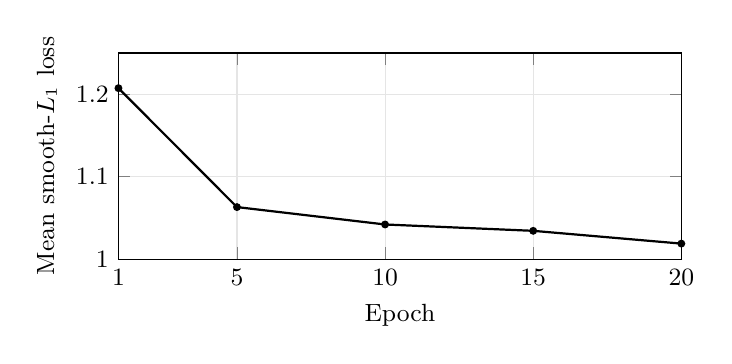
\begin{tikzpicture}
    \begin{axis}[
      width=0.72\linewidth, height=4.2cm,
      xlabel={Epoch}, ylabel={Mean smooth-$L_1$ loss},
      xmin=1, xmax=20, ymin=1.0, ymax=1.25,
      xtick={1,5,10,15,20},
      tick label style={font=\small}, label style={font=\small},
      grid=major, grid style={gray!20},
    ]
      \addplot[thick, mark=*, mark size=1pt] coordinates {
        (1,1.2074) (5,1.0632) (10,1.0421) (15,1.0344) (20,1.0189)
      };
    \end{axis}
  \end{tikzpicture}
  \caption{Per-epoch mean prediction loss for the behavioral predictor
  (HD-EPIC~P01, ViT-L, 20 epochs). The loss falls from $1.207$ to $1.019$ but is
  essentially flat after epoch~5, indicating an early feasibility ceiling rather
  than a training failure. Intermediate points ($1.063$, $1.042$, $1.034$) are
  the epoch~5/10/15 means. The curve is drawn from the five recorded checkpoints.}
  \label{fig:loss}
\end{figure}

% ------------------------------------------------------------
\subsection{Controls: separating token count from content}
\label{subsec:controls}

A conditioned run differs from an unconditioned one in more than the presence of
the behavioral signal. To expose anticipatory content, the probe is fed not only
the encoder's \num{1568} output tokens ($T\cdot N = 8\times196$) but also the
predictor's last predicted-frame block appended alongside them, taking the probe
input to \num{1764} tokens ($(T{+}1)\cdot N = 9\times196$). A naive
conditioned-versus-unconditioned comparison therefore confounds any content
effect with the effect of simply giving the probe more tokens. We break the
confound with a control family that holds the target constant and varies only
what fills the appended block:
\begin{itemize}
  \item \textbf{6a, encoder only} (\num{1568} tokens): no appended block.
  \item \textbf{6b, zero padding} (\num{1764} tokens): the appended block is zeros.
  \item \textbf{6c, content-free repeat} (\num{1764} tokens): the appended block
        repeats an existing frame, matching the token count without adding
        information.
  \item \textbf{Behavioral} (\num{1764} tokens): the appended block is the real
        prediction from the behaviorally-conditioned predictor.
\end{itemize}
The attentive pooler used for readout carries no positional encoding in its
attention path at any probed depth, so it is permutation-invariant over the token
axis, which is what makes 6b and 6c valid token-count-matched controls. We show
the controls before the headline comparison because the null only means something
once the token-count effect has been subtracted out.

The comparison is in Table~\ref{tab:main}, and the headline reading is best-epoch,
where the behavioral arm does not separate from its token-count-matched controls:
the behavioral-minus-6a gap is $-0.013$\,pp. Whatever advantage conditioning
appears to give is a token-count effect, not a content effect. The final-epoch
column tells a superficially different story that we address directly below, so
that it is not misread.

\begin{table}[t]
  \caption{Control family for the input-conditioning null (EK100 action R@5,
  \%, P01, signal-absent). Best-epoch values headline, with final-epoch
  (epoch~10) in parentheses. Best-epoch is the honest comparison, though it is
  selected on the reported validation set: the behavioral arm does not separate
  from its token-count-matched controls (behavioral $-$ 6a $= -0.013$\,pp). On
  final-epoch the behavioral arm leads by $0.15$--$0.27$\,pp, but only because it
  is the one arm that does not decay after epoch~8; that is a decay asymmetry, not
  a sign of the signal. The 6b and 6c conditions were run at two seeds, the third
  having been dropped once the direction was closed.}
  \label{tab:main}
  \centering
  \begin{tabular}{lccccc}
    \toprule
    Condition & Tokens & Seed 42 & Seed 43 & Seed 44 & Mean \\
    \midrule
    6a encoder only        & 1568 & 3.69 (3.38) & 3.44 (3.16) & 3.72 (3.54) & 3.62 (3.36) \\
    6b zero padding        & 1764 & 3.61 (3.61) & 3.59 (3.22) & ---         & 3.60 (3.42) \\
    6c content-free repeat & 1764 & 3.77 (3.46) & 3.31 (3.13) & ---         & 3.54 (3.29) \\
    Behavioral             & 1764 & 3.58 (3.48) & 3.49 (3.47) & 3.75 (3.75) & 3.61 (3.57) \\
    \bottomrule
  \end{tabular}
\end{table}

% ------------------------------------------------------------
\subsection{Five diagnostics on the frozen predictor}
\label{subsec:diagnostics}

Two readings of the null remained open after the controls: either the injection
pathway is too weak to expose whatever the signal carries, or the signal does
not carry action-relevant information at this horizon. The first recommends a
stronger architecture; the second recommends abandoning input-level conditioning
altogether. Rather than build a stronger pathway on the assumption that it would
help, we ran five diagnostics against the frozen predictor and the behavioral
signal directly (Table~\ref{tab:diagnostics}). They converge.

\begin{table}[t]
  \caption{Diagnostics bearing on whether a stronger pathway could recover
  anticipatory information. Full outputs in Appendix~\ref{sec:extended}.}
  \label{tab:diagnostics}
  \centering
  \small
  \begin{tabular}{lll}
    \toprule
    Diagnostic & Measurement & Interpretation \\
    \midrule
    Output shift (real vs.\ masked)      & relative $L_2 = 9.9\%$
      & the signal reaches the output \\
    Average-error gap (PEVA-1)           & $0.055\%$; real$>$masked 172/220, $p\approx3\times10^{-19}$
      & detectable but negligible \\
    Discrimination (PEVA-2)              & top-1 gap $0.0000$; 0/220 discordant
      & no discriminative margin \\
    Attention on the slot (Test A)       & $28.6\times$ (gaze) / $35.4\times$ (hand) uniform
      & the slot is heavily attended\dots \\
    Attention change, real vs.\ masked   & $\le 0.1\%$, negative in sign
      & \dots but indifferent to content \\
    Signal-alone anticipation (Test B)   & $12.2\%$ vs.\ $10.4\%$ prior ($+1.8$\,pp)
      & faint at source \\
    \bottomrule
  \end{tabular}
\end{table}

The attention result is the pivotal one. The predictor attends to the gaze and
hand slots at roughly twenty-nine to thirty-five times the uniform rate, so the
signal is clearly not being ignored on positional grounds. But replacing the real
signal with the mask token barely moves the attention; if anything the mask draws
marginally more. The model attends to where the signal sits and stays indifferent to what it says.
\S\ref{subsec:training-ablation} shows that this routing is
inherited from the action-conditioned pretraining rather than learned here, which
makes the absence of headroom a property of the architecture rather than of this
particular run. Key-biasing, the first mechanism a stronger, GazeQwen-style
pathway~\citep{pham2026gazeqwen} would add, needs headroom in exactly this
attention magnitude, and there is none to work with. Put beside the direct probe,
where the signal beats a class prior by only $1.8$ points, the reading is
consistent: the signal is registered but faint, and no rearrangement of the
pathway can recover information that a direct probe can barely find.

\begin{figure}[t]
  \centering
  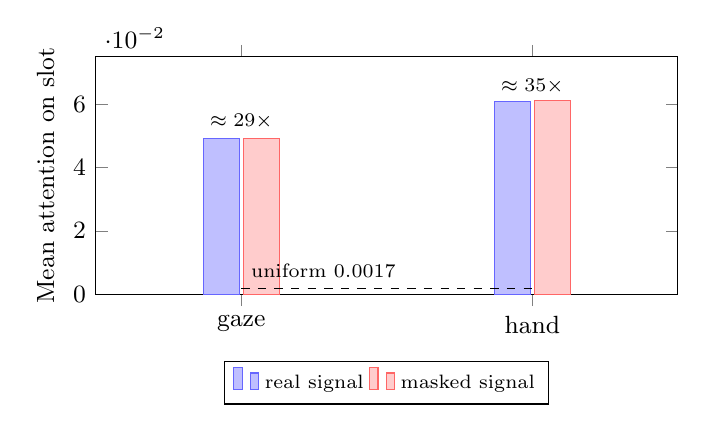
\begin{tikzpicture}
    \begin{axis}[
      width=0.74\linewidth, height=4.6cm,
      ybar=1.5pt, bar width=13pt,
      symbolic x coords={gaze, hand},
      xtick=data,
      ymin=0, ymax=0.075,
      ytick={0,0.02,0.04,0.06},
      ylabel={Mean attention on slot},
      enlarge x limits=0.5,
      tick label style={font=\small}, label style={font=\small},
      legend style={font=\scriptsize, at={(0.5,-0.28)}, anchor=north, legend columns=-1},
    ]
      \addplot[draw=blue!60, fill=blue!25] coordinates {(gaze,0.049080) (hand,0.060709)};
      \addplot[draw=red!60, fill=red!20]  coordinates {(gaze,0.049155) (hand,0.061035)};
      % uniform baseline, labelled
      \addplot[black, dashed, sharp plot, update limits=false]
        coordinates {(gaze,0.001716) (hand,0.001716)};
      \node[font=\scriptsize, anchor=south west] at (axis cs:gaze,0.0022) {uniform $0.0017$};
      % multiples above each pair
      \node[font=\scriptsize] at (axis cs:gaze,0.0545) {$\approx 29\times$};
      \node[font=\scriptsize] at (axis cs:hand,0.0655) {$\approx 35\times$};
      \legend{real signal, masked signal}
    \end{axis}
  \end{tikzpicture}
  \caption{Attention on the behavioral slots, real versus masked signal, against
  the uniform baseline (dashed, $0.0017$). Both slots draw roughly $29$--$35\times$
  uniform attention, yet the real and masked bars are indistinguishable
  (gaze $0.0491$ vs.\ $0.0492$; hand $0.0607$ vs.\ $0.0610$): the predictor
  attends to where the signal sits, not to what it says.}
  \label{fig:attention}
\end{figure}

% ------------------------------------------------------------
\subsection{Varying the training instead of the input}
\label{subsec:training-ablation}
\contrib{lead: Erfan}

Every diagnostic in \S\ref{subsec:diagnostics} holds one predictor fixed and
varies what is fed to it. That instrument can establish whether the model
responds to the signal, but it cannot separate the value of the information from
the cost of withholding an input the model was organised around: both appear as
the same difference. Separating them requires varying the \emph{training}. The
experiments below do exactly that, and they do it on the same warm-start
checkpoint that carries every anticipation result above
(\S\ref{subsec:method-setup}): its training run is re-executed with the
behavioral signal ablated, and the two models are compared directly. They are
scored on the conditioning objective, feature-space prediction error over
held-out participant~P08, on a fixed set of \num{96} clips, paired throughout.

\paragraph{The pathway is alive, graded, and small.}
Holding the video fixed and perturbing the gaze input by a known angle gives a
response that is monotone and near-linear from $1^\circ$ to $10^\circ$
($0.0012 \rightarrow 0.0024 \rightarrow 0.0061 \rightarrow 0.0130$, a factor of
eleven in output movement for a factor of ten in angle) and super-linear beyond,
reaching $0.081$ at $45^\circ$, about $14\%$ of the movement caused by
replacing the entire visual context. An identity control, the same forward pass
run twice, is exactly zero on all \num{96} clips, so every non-zero figure above
is signal rather than nondeterminism. The first reading of the null, that the
signal never reaches the predictor or that the pathway failed to train, is
therefore false. The channel functions; its gain is simply small.

\paragraph{Attention, quantified.}
On a $258$-token sequence the uniform share of a visual token's attention falling
on the gaze token is $1/258 = 0.388\%$. Measured, visual tokens spend
$12$--$26\%$ of their attention there, and in one head the gaze token takes
essentially the entire attention mass, $258\times$ uniform. The same
measurement on the \emph{untrained} model (action-conditioned weights, randomly
initialised projectors, no fine-tuning) already gives roughly $38\times$
uniform, and three epochs of training move it only to about $42\times$. The
routing is inherited from the action-conditioned pretraining that placed robot
action and state tokens in that position; training barely touches it.

\paragraph{Training built the pathway up, not down.}
A natural explanation for a null is that optimisation suppressed the new channel.
It did the opposite: the gaze projector's weight norm \emph{grew} $15.7\%$ against
its initialisation while every other trained parameter under the same weight decay
stayed within $0.05\%$ of its own.\footnote{The mask-token baseline used
throughout is itself a choice worth bounding. On the same checkpoint and clips the
conditioning gap is $+0.0007$ against mean imputation, $+0.0011$ against the mask
token and $+0.0022$ against zeros, a spread of $0.0015$ that is wider than the
smallest of the three effects.}

\paragraph{Most of what the projector learned is a constant.}
The mechanism behind the null is visible in the projector's parameters. Its bias
moved from exactly $0.000$ to $0.572$ against a weight norm of $1.270$, so a large
share of what it learned does not depend on gaze at all. That accounts for the pattern the
input-side diagnostics see: masking gaze moves the
prediction $5.2\times$ further than replacing it with a \emph{different} clip's
gaze ($0.084$ versus $0.016$). The model separates ``some gaze'' from ``no gaze''
far more sharply than one gaze from another, which is how heavy attention
coexists with small sensitivity: the heavily attended token is mostly a constant.\footnote{Shuffling gaze across time within a clip, which preserves the
marginal distribution and destroys the temporal correspondence, moves the
prediction by $1.5\%$ of a video swap and costs $+0.0004$ MSE.}

\paragraph{What the fine-tune was actually worth.}
Architecture and domain adaptation can be separated from conditioning too. The
stock action-conditioned predictor is $0.125$ MSE worse than the fine-tuned model
running with \emph{no} conditioning at all, on $96$ of $96$ clips, while gaze and
hand together are worth $0.0011$. Conditioning accounts for roughly $0.9\%$ of
what fine-tuning achieved; the remaining $0.125$ of $0.126$ is domain adaptation.

\paragraph{The matched information control.}
Finally, the warm-start checkpoint's own training run was repeated with the
behavioral signal dropped at every step, producing a predictor that has never
seen gaze or hand and is otherwise matched configuration-for-configuration. The
two were scored on the identical clips. Run with real signals, the signal-trained
model beats its own
masked condition by $\Delta = 0.0011$ ($p = 0.0015$); measured against the
never-conditioned model, the same real-signal predictor gains
$\Delta = 0.0003$ ($p = 0.40$, n.s.). The first quantity is the cost of
withholding an expected input; only the second is the value of the information,
and it is null. Two details sharpen it. Under masked evaluation the
never-conditioned model is in fact slightly \emph{better} ($-0.0008$,
$p = 0.015$), and feeding real gaze to a model that never saw one costs $+0.082$
on $96$ of $96$ clips. The signal is a large perturbation to a network not built
around it, and no help to one that was.

% ------------------------------------------------------------
\subsection{Decision: retiring the strong pathway at the design stage}
\label{subsec:b4}

The diagnostics of \S\ref{subsec:diagnostics} and
\S\ref{subsec:training-ablation} settle the weak-pathway-versus-faint-signal question in
favour of the faint signal, and we acted on that by retiring the stronger pathway
before building it. The ordering was deliberate and followed supervision. We took
the mechanism-adaptation reading of GazeQwen~\citep{pham2026gazeqwen}, adapting
its key-biasing and bottleneck-resampler mechanisms into our own predictor,
rather than reproducing its pipeline wholesale, and we ran the discriminating
diagnostic before spending anything on implementation.\footnote{The stronger
pathway was designed but never built: its forward pass raises rather than
silently running a partial implementation (Appendix~\ref{sec:code}). Since it was
never built, retiring it saved construction cost rather than discarding finished
work, and the design stays on record in case the binding constraint of
\S\ref{subsec:ddn} is relieved.}

There is a useful consequence to keeping the design around. A gate initialised at zero, left to train, would settle at zero
precisely if the model found the signal unhelpful, so the retired design doubles
as a falsifier rather than a dead end (\S\ref{subsec:method-strong}). One
qualification follows from \S\ref{subsec:training-ablation}: a settled-at-zero
gate is not the only informative outcome, since the existing projector was not
suppressed by training but grew, and still bought nothing. A gate could likewise
open onto a channel that carries little.

% ------------------------------------------------------------
\subsection{A motion-specific residual, and its limits}
\label{subsec:dissociation}

The aggregate signal is faint, but the direct probe is not uniform across
targets. Split by verb and noun, gaze and hand beat vision on \emph{verbs}, which
encode motion, and lose to it on \emph{nouns}, which encode object identity:
vision reaches $0.480$ on verbs against the signal's $0.594$, and $0.318$ on
nouns against the signal's $0.231$. Put plainly, the behavioral signal anticipates
how the hand will move, not what it will act on, and object identity is what makes
the EK100 action space hard. The same verb/noun split turns out to be the
organising principle of the two strongest published EK100 systems, both
frozen-V-JEPA-2.1 probes, which separate their verb and noun heads on the same
reasoning that verbs track motion and nouns track object
appearance~\citep{chu2026jfaa, wang2026tapjepa}. So the dissociation is not a
quirk of our setup.

This one encouraging result warranted a more careful test than the exploratory
probe that produced it. We evaluated it as a held-out verb-level anticipation
probe on HD-EPIC~P01, comparing the behavioral arm against a vision arm and
against the verb class prior across horizons. An initial version was discarded
on two grounds: the seeds were inert, because zero-initialised weights under
full-batch deterministic optimisation consume no randomness, and model selection
read the reported validation set. The corrected version restores genuine seed
variance through bootstrap resampling and reports on a held-out test split; a
final (fair-vision) version additionally fits the vision arm under an a-priori
grid with a prior-mimicry guard, so the comparator cannot pass by collapsing
onto the class marginal. Results are in Table~\ref{tab:dissociation}.

\begin{table}[t]
  \caption{Verb-level behavior-minus-vision margins on held-out test data
  (fair-vision, v3). The one-second row is a separate run with its own subsample
  and prior and is not directly comparable to the longer horizons. An earlier dissociation figure, computed against an under-fit vision comparator, is superseded by these values and is not reported.}
  \label{tab:dissociation}
  \centering
  \begin{tabular}{lccl}
    \toprule
    Horizon & behavior $-$ vision & 95\% CI & behavior vs.\ prior \\
    \midrule
    1\,s  & $+0.035$ & $[+0.008, +0.118]$ & $-0.051$ (below) \\
    3\,s  & $+0.054$ & $[-0.029, +0.099]$ & $-0.092$ (below) \\
    5\,s  & $+0.103$ & $[+0.017, +0.144]$ & $-0.060$ (below) \\
    10\,s & $+0.121$ & $[+0.054, +0.169]$ & $-0.059$ (below) \\
    \bottomrule
  \end{tabular}
\end{table}

Two qualifications are decisive. First, once the vision arm is fitted fairly, a
substantial part of what had looked like a behavioral advantage turns out to have
been an under-fit comparator: at the three-second horizon roughly half the
exploratory margin disappears, and the earlier headline figure should not be
quoted. Second, and
more fundamentally, the behavioral arm never exceeds the verb class prior at any
horizon; the margins against the prior are uniformly negative. This is a
dissociation below the level of useful anticipation, not anticipation itself. The margin does widen with horizon, but the
widening should not be read as the signal strengthening. From three to ten
seconds it grows by $0.067$, of which roughly half is the vision comparator
decaying ($0.530\rightarrow0.495$) and roughly half the behavioral arm rising
($0.583\rightarrow0.616$). Both arms move, and the behavioral arm stays beneath
its own class prior at every horizon, which is the fact that bounds the claim.

% ------------------------------------------------------------
\subsection{The binding constraint: sample size, not dynamic range}
\label{subsec:ddn}

A natural objection is that probe accuracies so far below published EK100
baselines leave too little dynamic range to detect anything, so that we are
seeing a floor artifact. The evidence points the other way, to a ceiling in
sample size. The HD-EPIC verb probe trains on roughly \num{1900} examples, the
verb-labelled subsample of P01 used for this analysis, which is a different and
much smaller set than the EK100 clip counts of \S\ref{subsec:protocol}. On that
set both arms interpolate their training data: vision reaches a training recall
near unity, the behavioral arm around $0.80$. This is the familiar
high-dimension, low-sample regime, where no amount of optimiser tuning buys
generalisation. Two observations rule out a pure floor. First, the noun contrast
reverses the sign of the verb contrast, and a uniform floor cannot produce a sign
reversal. Second, as \S\ref{subsec:protocol} established, the evaluation is
single-participant, which both explains the narrow between-seed spread and points
to the concrete fix. The honest limitation is single-participant sample size, and
\S\ref{sec:conclusion} takes up the remedy.

% ------------------------------------------------------------
\subsection{Horizon analysis: how far ahead the signal is legible}
\label{subsec:horizon}
\contrib{lead: Erfan}

The diagnostics so far ask what the predictor does with the behavioral signal at
one horizon. This subsection asks a complementary question about the signal
itself: over what lead time is behavioral information present in the frozen
representation at all? The measurement is not anticipation recall and must not be
read against Table~\ref{tab:main}. From the frozen encoder's features at time
$\tau$ we regress a behavioral target at $\tau + t$ with a ridge probe, and report
\emph{skill}, the fractional reduction in squared error against a
predict-the-mean baseline: zero is chance, one is exact. Data are
HD-EPIC~\citep{perrett2025hdepic} recordings. Because each participant has their
own kitchen, we separate a split across held-out \emph{recordings} (same people,
unseen scenes) from a split across held-out \emph{participants} (unseen people),
and carry a hand-pose target alongside gaze as a positive control.

\begin{table}[t]
  \caption{Recoverability of behavioral targets from the frozen encoder as a
  function of lead $t$ (skill; $0$ = chance). Gaze is near chance across held-out
  participants at every lead, while palm position, regressed from the same
  features under the same split, transfers and then decays. Whatever behavioral
  information the representation carries is about the present.}
  \label{tab:horizon}
  \centering
  \begin{tabular}{lccc}
    \toprule
    & \multicolumn{2}{c}{gaze} & hand (control) \\
    \cmidrule(lr){2-3}\cmidrule(lr){4-4}
    Lead $t$ & held-out participants & held-out recordings & held-out participants \\
    \midrule
    $0.00$\,s & $+0.001$ & $+0.116$ & $+0.346$ \\
    $0.25$\,s & $+0.004$ & $+0.071$ & $+0.287$ \\
    $0.50$\,s & $-0.015$ & $+0.055$ & $+0.207$ \\
    $1.00$\,s & $-0.007$ & $-0.000$ & $+0.079$ \\
    $2.00$\,s & $-0.027$ & $+0.015$ & $-0.032$ \\
    \bottomrule
  \end{tabular}
\end{table}

Three readings follow, in order of how much they constrain the rest of the paper.

\textbf{Gaze is not redundant with what the encoder already represents.} A
natural way to dismiss the null of \S\ref{subsec:controls} is to say that people
look at salient objects, salient objects are visible, and so the gaze token tells
a visual encoder nothing it does not already have. Table~\ref{tab:horizon} rules
that out: across held-out participants gaze is recoverable at skill $0.001$ even
at zero lead, indistinguishable from chance. The conditioning signal is not
redundant, which makes the null harder to explain away rather than easier.

\textbf{The collapse is specific to gaze, not an artifact of the probe or the
domain gap.} Under the identical split, features and probe, palm position retains
skill $0.346$ across unseen participants. Participant identity is itself
recoverable from these features at $88.7\%$ (seven-way, chance $14.3\%$), so the
domain gap between kitchens is real and large --- and a behavioral target crosses
it anyway. The probe can decode behavior from this representation; it is gaze
specifically that does not survive a change of person.

\textbf{The horizon reading proper: behavioral legibility is a present-tense
property.} Palm skill falls from $0.346$ at zero lead to $0.079$ at one second and
to chance by two. Gaze, in the one split where it is measurable at all, falls from
$0.116$ to zero over the same interval. Whatever the frozen representation knows
about behavior, it knows about now, and that knowledge is largely gone by the
one-to-two-second mark --- the horizon at which this paper's anticipation
experiments run.

We are explicit about what this does not show. It characterises the decay of
behavioral legibility with lead; it is not evidence that behavioral conditioning
becomes \emph{more} valuable at longer horizons. The widening margin of
\S\ref{subsec:dissociation} is a different measurement with its own explanation,
and neither published challenge system sweeps horizon at
all~\citep{chu2026jfaa, wang2026tapjepa}, so there is no external support for a
growth reading. If anything the evidence here runs the other way: the signal is
most legible at the shortest leads, which bounds what any input-level pathway
could have delivered at the horizon we probe.

% ============================================================
% 5. DISCUSSION -- humanized. Cut self-congratulation ("worth naming",
% "we think one of the transferable lessons"). GABRIL: state direction,
% drop the second-hand-ness advertisement (fix #4).
% ============================================================
\section{Discussion}

\paragraph{What the null does and does not say.}
The central result is a null with a mechanism behind it. Conditioning a frozen
V-JEPA~2 predictor on gaze and hand at the input does not improve short-horizon
anticipation, and the five diagnostics say why: the signal reaches the
predictor's output, the predictor does not respond to its content, and on its own
the signal predicts the next action barely above a class prior. So the claim we
are entitled to is narrow. Not that gaze and hand are uninformative, but that at
this horizon, this sample size, and through this pathway they carry too little
action-relevant information to move the prediction. That narrower claim matters,
because it points to a different fix than ``build a bigger pathway.''

\paragraph{Detectability versus decision-relevance.}
A single accuracy number hides a distinction the PEVA-style readout makes
visible. One question is whether the signal is detectable at all; another is
whether it is large enough to change a decision. Here the signal is detectable in
the statistical sense (it beats the masked version on 172 of 220 clips) yet
produces no discriminative margin (not one discordant pair). An effect that is
real but decision-irrelevant is easy to report as a success if only average error
is measured, which is one reason we ran both stages of the readout rather than
the first alone.

\paragraph{The motion/object dissociation, in context.}
The one piece of residual structure is that gaze and hand favour verbs while
vision favours nouns. The natural reading is that behavioral signals encode how
the body is about to move rather than what it will act on, and that EK100 is hard
mainly because of object identity. As a performance result this carries little
weight, since it sits below the verb prior. As corroboration it carries more: the
two strongest published EK100 systems independently split their probes along the
same verb/noun line and defend it with the same motion-versus-appearance argument
\citep{chu2026jfaa, wang2026tapjepa}. When three separate efforts land on the
same boundary, it is likely a property of the task rather than of our setup.

\paragraph{Why input-level conditioning may be the weak use of these signals.}
Set against the recent literature, our null looks less like a surprise and more
like one more instance of a pattern. Methods that use gaze to \emph{supervise} a
representation during training and then drop it at inference tend to report gains
where input concatenation, as here, does not: the gaze regulariser of
GABRIL \citep{banayeeanzade2025gabril}, the gaze-regularised vision-language
models of \citet{pani2026gazereg}, and the goal-consistency objective of
\citet{royfernando2022abstractgoal} all take this route. GazeQwen puts the point
directly, arguing that the obstacle is a missing learned pathway from gaze into
the model's internal representations rather than any deficit in the signal. Our
diagnostics fit that argument at the input level almost exactly: the model
attends to where the signal sits but not to what it says, which is what a missing
learned pathway would look like.

\paragraph{Relation to the horizon analysis.}
The horizon sweep of \S\ref{subsec:horizon} measures something different from the
margins above: how far ahead a behavioral target is recoverable from the frozen
representation at all. It finds that behavioral legibility is a present-tense
property, largely gone by one to two seconds, which bounds what any input-level
pathway could have delivered at the horizon we probe. One caution keeps the two
analyses consistent. The behavior-minus-vision margin in \S\ref{subsec:dissociation} does widen with
horizon, but the widening splits roughly evenly between a decaying vision
comparator and a rising behavioral arm, and the behavioral arm remains below its
own class prior at every horizon. Since neither published challenge system sweeps
horizon, there is no outside evidence for a ``signal grows with horizon'' reading
either. The
horizon numbers describe the regime; they are not evidence that a longer horizon
rescues the signal.
% ============================================================
% 6. LIMITATIONS -- humanized. Strong section already; just vary cadence,
% cut em-dashes, let some sentences be plain.
% ============================================================
\section{Limitations}

We put the limitations before the discussion's conclusions travel too far,
because several of them set exactly how far those conclusions can go.

\paragraph{Single-participant evaluation.}
The binding limitation is scope. The EK100 probe was evaluated on P01 alone
(\num{870} validation clips), and the HD-EPIC direct probes use P01 as well.
\S\ref{subsec:protocol} explains that this followed from which videos were on disk
at run time rather than from a deliberate choice. Every anticipation claim in the paper is therefore a claim about one
participant. Two analyses are exceptions and should be read as such: the
training-side ablations of \S\ref{subsec:training-ablation} and the
recoverability probes of \S\ref{subsec:horizon} train on P01--P07 and evaluate
on held-out participants, so where our conclusion rests on those it is not
single-participant. We make no assertion about
cross-participant generalisation, and the small spread between seeds should be
read as a single-participant artifact, not as evidence of stability across the
dataset.

\paragraph{Sample size below the generalisation threshold.}
Participant count aside, the direct probe runs on about \num{1900} training
examples against a high-dimensional input, and both arms interpolate that
training set (\S\ref{subsec:ddn}). In that regime held-out performance is set by
sample size, not by model or optimiser choices. This is why we call the result a
faint signal under a sample ceiling rather than no signal at all: the experiment
as run cannot separate a genuinely absent effect from a real one too small to
show at this $n$.

\paragraph{Mechanism claims rest on the direct probe, not the benchmark.}
The dissociation and the signal-content diagnostics come from the signal-present
HD-EPIC venue. The EK100 result is signal-absent by construction, since the
behavioral slots are masked at evaluation, so it speaks to whether a
behaviorally-trained predictor transfers, not to the gaze/hand-to-motion
mechanism. We do not carry evidence across that line. The cost of that discipline
is that our mechanism claims are never checked on the benchmark task itself.

\paragraph{The vision comparator sits below its own prior.}
Even fitted fairly (\S\ref{subsec:dissociation}), the vision arm does not clear
the verb class prior non-degenerately, and the behavioral arm never clears it at
all. The dissociation is established below the level of useful anticipation. A
stronger comparator, or a task with more headroom above the prior, might change
its size, though on this evidence not its sign.

\paragraph{The stronger pathway was not run.}
We retired the GazeQwen-informed pathway at the design stage
(\S\ref{subsec:b4}) on the strength of the diagnostics, without implementing it.
The diagnostics argue convincingly that it would not recover the signal, but the
argument is inferential. We did not falsify it directly, and a zero-initialised
gated implementation is still the clean way to do so if the sample-size
constraint is ever lifted.

\paragraph{The signal-drop control is scored on the conditioning objective, not on EK100.}
The matched never-conditioned control of \S\ref{subsec:training-ablation} is a
full-rate ablation of the very checkpoint that carries every anticipation result
here, which is stronger than a comparison across models. It is scored, however, on
feature-space prediction error over a held-out participant rather than through the
EK100 probe itself. What remains unrun is the same ablation carried all the way
through to anticipation recall; we therefore report the null in signal content as
established on the conditioning objective and inherited, rather than
independently re-measured, downstream.

\paragraph{The checkpoint is under-trained relative to the intended scale.}
Every anticipation number here rests on a predictor fine-tuned for three epochs at
thirty clips per recording (\S\ref{subsec:method-setup}). That is the small
configuration, not the scale the conditioning study was designed around, and no
full-scale run ever completed. This matters in a specific direction: a null
measured on an under-trained predictor is weaker evidence than it reads as,
because a model that has not finished learning the task has not finished learning
what to do with an auxiliary input either. Two things limit how much weight this
objection can carry. The feasibility curve of \S\ref{subsec:protocol} is
essentially flat after the fifth epoch, and the fine-tune is demonstrably worth
$0.125$ MSE over the stock predictor (\S\ref{subsec:training-ablation}), so the
training did take. But we cannot rule out that a longer schedule would give the
conditioning pathway something it currently lacks, and we do not claim otherwise.

\paragraph{Goal-level probing is infeasible on one participant.}
The representation-level test we wanted to run, a recipe-goal probe on
HD-EPIC~P01, does not work at single-participant scale. Under the hand-validity
session split, four of eight recipes have no held-out examples, one recipe
accounts for about three-quarters of the held-out set, and recipe identity is
nearly collinear with session identity. That is a characterised data requirement
rather than a failed experiment, and it is what motivates the multi-participant
direction of \S\ref{sec:conclusion}.
% ============================================================
% 7. CONCLUSION -- humanized. Short, plain.
% ============================================================
\section{Conclusion}\label{sec:conclusion}

We asked whether conditioning a frozen V-JEPA~2 predictor on egocentric gaze and
hand improves short-horizon action anticipation, and when it did not, we asked
why. For one participant at a one-to-two-second horizon on the benchmark, and across
held-out participants on the conditioning objective, the answer is that the
signal reaches the predictor but does not change its output in any
content-dependent way. Feeding these signals in at the input is the weak way to
use them. We retired a stronger conditioning pathway at the design stage on
converging diagnostic evidence, described a motion-specific residual that lives
below the level of useful anticipation, and traced the binding constraint to
single-participant sample size rather than to any floor in the probe's dynamic
range.

\paragraph{Future work.}
The evidence points not toward a stronger input pathway but toward a different
use of the signal: supervising the representation with gaze and hand during
training and discarding them at inference, aimed at goal- or intention-level
targets rather than the next action. To our knowledge that intersection is still
open, a frozen-JEPA latent predictor trained with a representation-level
auxiliary loss on behavioral signals against a goal-level target, and it is the
natural next step from here. It also needs the goal probe run across participants rather than within one.
HD-EPIC~P01--P07 already underpins the conditioning experiments reported here
(\S\ref{subsec:training-ablation}); extending the recipe-level probe to that
range is what our single-participant attempt shows to be a prerequisite rather
than a convenience.

% ============================================================
% ACKNOWLEDGMENTS
% ============================================================
\begin{ack}
We thank Jun.-Prof.\ Dr.-Ing.\ Stefan L\"udtke for overseeing the project.
We also thank Ashwin Nedungadi, and Kl\'ara Orb\'an for supervising the Rostock
and Cluj teams, respectively, and for their guidance and feedback throughout the
project.

We used AI assistants (Anthropic's Claude, including Claude Code) during this
project. Their role was drafting and editing assistance, code scaffolding and
execution on the compute cluster, literature retrieval, and help organising and
reconciling experimental records. All research questions, experimental designs,
decisions, and interpretations are the authors' own, and all reported
experimental results were verified by the authors against primary experimental
evidence. The authors take full responsibility for the content of this report.
\end{ack}

% ============================================================
% REFERENCES
% ============================================================
\bibliographystyle{plainnat}
\bibliography{references}

%%%%%%%%%%%%%%%%%%%%%%%%%%%%%%%%%%%%%%%%%%%%%%%%%%%%%%%%%%%%
\appendix
%%%%%%%%%%%%%%%%%%%%%%%%%%%%%%%%%%%%%%%%%%%%%%%%%%%%%%%%%%%%

% ============================================================
% APPENDIX A: CONTRIBUTION STATEMENT (mandatory; refs/appendix don't count to 15pp)
% ============================================================
\section{Contribution statement}
\label{sec:contrib}

The authors contributed to distinct, complementary workstreams under a shared
research goal. This report was written by Parsa and Erfan; Ioana is a project
collaborator whose contributions inform the work but who did not author this
report.

\paragraph{Seyyed Parsa Sharifi.}
Designed and directed the diagnostic study of the conditioning pathway: the EK100
anticipation probe of the behaviorally-trained predictor and its 6a/6b/6c control
family; the bit-exact verification of the weak (peer-token) pathway; the
silent-null gradient guard; the five diagnostics (output shift, PEVA-1/2,
attention Test~A, direct-probe Test~B); the verb/noun dissociation analysis and
its fair-vision correction; and the $d\gg n$ sample-size analysis. Specified the
stronger (GazeQwen-informed) pathway and made the design-stage decision to retire
it. Proposed the diagnostic-first approach adopted under supervision. Led the writing of the Method, Experiments, Discussion, Limitations, and Conclusion, and assembled the report.

\paragraph{Erfan Yekehzare.}
Authored the JEPA/VL-JEPA background (\S\ref{subsec:bg-jepa}) and the horizon
analysis (\S\ref{subsec:horizon}), including the frozen-feature recoverability
probes and the hand-pose transfer control they report. Designed and built the ego predictor that integrates
the behavioral projection layers, together with its fine-tuning and evaluation
pipeline, and trained the ViT-G behavioral checkpoint on which every anticipation
result in this report is based. Built and ran the companion conditioning track
that supplies the matched never-conditioned control and the untrained-model
attention measurement of \S\ref{subsec:diagnostics}.

\paragraph{Ioana Marica (collaborator, non-author).}
Contributed the representation- and signal-level hypotheses, an initial
implementation of the gaze and hand projection layers and their token
construction, the encoder-supervision direction, and the PEVA evaluation idea. These inform the framing and future-work
direction of this report; Ioana did not author the report itself.
% ============================================================
% APPENDIX B: EXTENDED EXPERIMENTS  (outside 15-page limit)
% Filled from Notion mirror + Part III PDF. Sample-size FLAG on dissociation n.
% ============================================================
\section{Extended experimental details}
\label{sec:extended}

\subsection{Full control-family seed table}
Table~\ref{tab:main} in the main text reports best-epoch (final-epoch in
parentheses). For completeness: condition means over available seeds are, best /
final, Phase~5 $3.606 / 3.567$; 6a $3.619 / 3.360$; 6b $3.601 / 3.415$; 6c
$3.544 / 3.294$. All values are EK100 action R@5 (\%), P01, signal-absent
evaluation, read from the per-run evaluation CSVs (five-decimal precision;
cross-checked against the tqdm logs). The 6b and 6c seed-44 runs were not
launched once the direction was closed, so those two conditions have two seeds.

\subsection{PEVA stage-1 and stage-2 statistics}
Stage-1 (average-error), $N=220$: mean relative gap $0.00055$; the real signal
beats the masked signal on $172/220$ clips ($78.2\%$); Wilcoxon
$p = 3.15\times10^{-19}$. Stage-2 (discrimination), $N=220$: top-1 error
identical for real and masked ($0.9545$; chance $0.0625$); McNemar both-correct
$210$, real-only $0$, masked-only $0$, both-wrong $10$; margin-$L_2$ Wilcoxon
$p = 2.46\times10^{-24}$. The two stages together give the detectable-but-not-
decision-relevant decoupling discussed in \S\ref{subsec:diagnostics}.

\subsection{Diagnostic raw outputs}
Output shift: $L_2(\text{real},\text{masked}) = 225.35$, $\lVert\text{real}\rVert
= 2272.18$, relative $L_2 = 0.0992$. Test~A (attention; uniform baseline
$0.001716$): gaze real $0.049080$ ($28.6\times$) vs.\ masked $0.049155$; hand
real $0.060709$ ($35.4\times$) vs.\ masked $0.061035$; real $>$ masked is false
for both. Test~B (direct probe; class-prior R@5 $= 0.1053$, chance $0.0041$),
per-target R@5 (vision, behavior, prior): action $0.1137 / 0.1216 / 0.1039$;
verb $0.4804 / 0.5941 / 0.6137$; noun $0.3176 / 0.2314 / 0.3000$. Note the verb
prior ($0.6137$) exceeds both arms: the behavioral advantage on verbs is relative
to vision, not to the prior.

\subsection{Verb/noun dissociation, all horizons}
Horizon sweep (fair-vision v3, common set), verb R@5 with verb prior $0.6749$:
3\,s behavior $0.5830\pm0.0108$, vision $0.5295\pm0.0305$, margin $+0.0535$
$[-0.0288, +0.0988]$; 5\,s $0.6145\pm0.0229$ vs.\ $0.5117\pm0.0118$, $+0.1029$
$[+0.0165, +0.1440]$; 10\,s $0.6159\pm0.0085$ vs.\ $0.4952\pm0.0216$, $+0.1207$
$[+0.0535, +0.1687]$. One-second row (separate subsample, prior $0.5922$):
behavior $0.5412\pm0.0096$, vision $0.5059\pm0.0169$, margin $+0.0353$
$[+0.0078, +0.1176]$. The earlier figure computed against the under-fit vision comparator is superseded by these values.
% FLAG: test-set n for the v3 common set -- Part III states 762; the reconstructed
% experiment log gives 243 for Option 2 v2 (with a known Notion 243->1. corruption
% now fixed). Confirm which n attaches to which row before stating a sample count.

\subsection{\texorpdfstring{$d \gg n$}{d >> n} comparator diagnostic}
In the signal-present HD-EPIC probe both arms interpolate their training data:
vision reaches training R@5 near unity while test R@5 sits at $0.50$--$0.62$; the
behavioral arm reaches training R@5 around $0.80$. A prior-mimicry guard voids any
run whose top-5 set collapses onto the class marginal (mean top-5 overlap
$\approx 1.0$). At roughly \num{1900} training examples the fair-vision pass-
condition fails at all four horizons, locating the constraint in sample size
rather than pathway design.
% ============================================================
% APPENDIX C: CODE SNIPPETS  (outside 15-page limit)
% Load-bearing excerpts, verbatim from the Part III appendix. Full source -> GitHub.
% ============================================================
\section{Selected code}
\label{sec:code}

Excerpts are the load-bearing pieces a reader might wish to verify; full source is
in the project repository (linked on the title page).

\subsection{Conditioning-mode switch and the unimplemented strong path}
The strong pathway is a declared but unimplemented switch point; its forward pass
raises rather than running a partial implementation
(\texttt{src/models/ego\_predictor.py}).
\begin{lstlisting}[language=Python]
_CONDITIONING_MODES = ("weak", "strong")
if conditioning_mode not in _CONDITIONING_MODES:
    raise ValueError(
        f"conditioning_mode must be one of {_CONDITIONING_MODES}, "
        f"got {conditioning_mode!r}")
self.conditioning_mode = conditioning_mode
...
if self.conditioning_mode == "strong":
    raise NotImplementedError(
        "conditioning_mode='strong' is a placeholder switch point -- not "
        "implemented. WEAK (peer-token concatenation) must be proven "
        "equivalent to the existing Phase 5 eval path before STRONG is built.")
\end{lstlisting}

\subsection{The weak path that runs --- peer-token concatenation}
\begin{lstlisting}[language=Python]
x = self.predictor_embed(x)
B, N_ctxt, D = x.size()
T = N_ctxt // (self.grid_height * self.grid_width)
gaze_tokens = self._encode_gaze(gaze_vecs, gaze_valid)      # (B, T, D)
hand_tokens = self._encode_hand(hand_vecs, l_valid, r_valid) # (B, T, D)
x = x.view(B, T, self.grid_height * self.grid_width, D)
x = torch.cat([gaze_tokens.unsqueeze(2),
               hand_tokens.unsqueeze(2), x], dim=2)
x = x.flatten(1, 2)  # (B, T*(H*W+2), D)
\end{lstlisting}

\subsection{Attention hook site for the (unbuilt) strong path}
The stock attention site where the strong pathway's key-biasing would attach
(\texttt{src/models/utils/modules.py}), shown to document the intended hook point.
\begin{lstlisting}[language=Python]
if action_tokens > 0:
    def merge_(tx, ta):
        tx = tx.view(B, self.num_heads, T, H * W, -1)
        ta = ta.view(B, self.num_heads, T, action_tokens, -1)
        return torch.cat([ta, tx], dim=3).flatten(2, 3)
    q = merge_(q, action_q)
    k = merge_(k, action_k)   # <- strong-mode key-bias would hook here
    v = merge_(v, action_v)
x = F.scaled_dot_product_attention(q, k, v, ...)
\end{lstlisting}

\subsection{Weak-mode equivalence check}
Output of the equivalence check
(\texttt{logs/weak\_equivalence\_2026-07-23/summary.md}): the new weak mode
matches the Phase-5 route to eight decimal places.
\begin{lstlisting}
IntegratedColleaguePredictor (Phase 5 route):
  shape [1,1568,1408] mean -0.01062952 std 1.52526128
  min -35.52310944 max 92.15590668
our weak-mode (masked):
  shape [1,1568,1408] mean -0.01062952 std 1.52526128
  min -35.52310944 max 92.15590668
max abs diff = 0.00000000 (threshold 1e-04)
mean abs diff = 0.00000000
verdict: MATCH
\end{lstlisting}

\subsection{Gradient-flow guard}
After one backward pass every unfrozen module is asserted to carry a non-zero
gradient; frozen blocks correctly carry none.
\begin{lstlisting}
dummy loss = 2.338494   unfreeze_last_n_blocks = 6
module                grad_norm   n_params  n_no_grad
gaze_proj             8.29e-01    2         0
hand_proj             5.45e-01    2         0
predictor_blocks.22   2.47e+00    12        0
predictor_blocks.23   2.60e+00    12        0
all watched modules non-zero: True
frozen spot check: blocks 0, 9, 17 -> requires_grad False, grad None
\end{lstlisting}
% ============================================================
% APPENDIX D: ABBREVIATIONS & NOTATION  (outside 15-page limit)
% Acronym-dense report -> a lookup table earns its place here, not in
% the front matter (which would cost page-limit space).
% ============================================================
\section{Abbreviations and notation}

\begin{table}[h]
  \centering
  \begin{tabular}{ll}
    \toprule
    Term & Meaning \\
    \midrule
    JEPA        & Joint-Embedding Predictive Architecture \\
    V-JEPA 2    & Video JEPA 2 (frozen encoder + latent predictor) \\
    V-JEPA 2-AC & \dots\ Action-Conditioned variant (robot signals) \\
    V-JEPA 2.1  & Dense-feature V-JEPA revision \\
    ViT-L / ViT-G & Vision Transformer, Large / Giant \\
    EK100       & EPIC-KITCHENS-100 \\
    HD-EPIC     & Highly-Detailed EPIC egocentric dataset \\
    R@5         & Recall at 5 \\
    RoPE        & Rotary Position Embedding \\
    PEVA        & Predicting Ego-centric Video from human Actions \citep{bai2025peva} \\
    WEAK        & Peer-token concatenation pathway (built) \\
    STRONG      & GazeQwen-informed fusion pathway (designed, not built) \\
    6a/6b/6c    & Control family (encoder-only / +zeros / +repeat) \\
    CI          & Confidence interval \\
    \bottomrule
  \end{tabular}
\end{table}
% Trim to what actually appears in the final text; add gaze/hand dims,
% signal_dropout, etc. if referenced by shorthand.


% ---- NeurIPS checklist (after refs + appendix; does NOT count to limit) ----
% \section*{NeurIPS Paper Checklist}

%%% BEGIN INSTRUCTIONS %%%
The checklist is designed to encourage best practices for responsible machine learning research, addressing issues of reproducibility, transparency, research ethics, and societal impact. Do not remove the checklist: {\bf The papers not including the checklist will be desk rejected.} The checklist should follow the references and follow the (optional) supplemental material.  The checklist does NOT count towards the page
limit. 

Please read the checklist guidelines carefully for information on how to answer these questions. For each question in the checklist:
\begin{itemize}
    \item You should answer \answerYes{}, \answerNo{}, or \answerNA{}.
    \item \answerNA{} means either that the question is Not Applicable for that particular paper or the relevant information is Not Available.
    \item Please provide a short (1--2 sentence) justification right after your answer (even for \answerNA). 
   % \item {\bf The papers not including the checklist will be desk rejected.}
\end{itemize}

{\bf The checklist answers are an integral part of your paper submission.} They are visible to the reviewers, area chairs, senior area chairs, and ethics reviewers. You will also be asked to include it (after eventual revisions) with the final version of your paper, and its final version will be published with the paper.

The reviewers of your paper will be asked to use the checklist as one of the factors in their evaluation. While \answerYes{} is generally preferable to \answerNo{}, it is perfectly acceptable to answer \answerNo{} provided a proper justification is given (e.g., error bars are not reported because it would be too computationally expensive'' or ``we were unable to find the license for the dataset we used''). In general, answering \answerNo{} or \answerNA{} is not grounds for rejection. While the questions are phrased in a binary way, we acknowledge that the true answer is often more nuanced, so please just use your best judgment and write a justification to elaborate. All supporting evidence can appear either in the main paper or the supplemental material, provided in appendix. If you answer \answerYes{} to a question, in the justification please point to the section(s) where related material for the question can be found.

IMPORTANT, please:
\begin{itemize}
    \item {\bf Delete this instruction block, but keep the section heading ``NeurIPS Paper Checklist"},
    \item  {\bf Keep the checklist subsection headings, questions/answers and guidelines below.}
    \item {\bf Do not modify the questions and only use the provided macros for your answers}.
\end{itemize} 
 

%%% END INSTRUCTIONS %%%


\begin{enumerate}

\item {\bf Claims}
    \item[] Question: Do the main claims made in the abstract and introduction accurately reflect the paper's contributions and scope?
    \item[] Answer: \answerTODO{} % Replace by \answerYes{}, \answerNo{}, or \answerNA{}.
    \item[] Justification: \justificationTODO{}
    \item[] Guidelines:
    \begin{itemize}
        \item The answer \answerNA{} means that the abstract and introduction do not include the claims made in the paper.
        \item The abstract and/or introduction should clearly state the claims made, including the contributions made in the paper and important assumptions and limitations. A \answerNo{} or \answerNA{} answer to this question will not be perceived well by the reviewers. 
        \item The claims made should match theoretical and experimental results, and reflect how much the results can be expected to generalize to other settings. 
        \item It is fine to include aspirational goals as motivation as long as it is clear that these goals are not attained by the paper. 
    \end{itemize}

\item {\bf Limitations}
    \item[] Question: Does the paper discuss the limitations of the work performed by the authors?
    \item[] Answer: \answerTODO{} % Replace by \answerYes{}, \answerNo{}, or \answerNA{}.
    \item[] Justification: \justificationTODO{}
    \item[] Guidelines:
    \begin{itemize}
        \item The answer \answerNA{} means that the paper has no limitation while the answer \answerNo{} means that the paper has limitations, but those are not discussed in the paper. 
        \item The authors are encouraged to create a separate ``Limitations'' section in their paper.
        \item The paper should point out any strong assumptions and how robust the results are to violations of these assumptions (e.g., independence assumptions, noiseless settings, model well-specification, asymptotic approximations only holding locally). The authors should reflect on how these assumptions might be violated in practice and what the implications would be.
        \item The authors should reflect on the scope of the claims made, e.g., if the approach was only tested on a few datasets or with a few runs. In general, empirical results often depend on implicit assumptions, which should be articulated.
        \item The authors should reflect on the factors that influence the performance of the approach. For example, a facial recognition algorithm may perform poorly when image resolution is low or images are taken in low lighting. Or a speech-to-text system might not be used reliably to provide closed captions for online lectures because it fails to handle technical jargon.
        \item The authors should discuss the computational efficiency of the proposed algorithms and how they scale with dataset size.
        \item If applicable, the authors should discuss possible limitations of their approach to address problems of privacy and fairness.
        \item While the authors might fear that complete honesty about limitations might be used by reviewers as grounds for rejection, a worse outcome might be that reviewers discover limitations that aren't acknowledged in the paper. The authors should use their best judgment and recognize that individual actions in favor of transparency play an important role in developing norms that preserve the integrity of the community. Reviewers will be specifically instructed to not penalize honesty concerning limitations.
    \end{itemize}

\item {\bf Theory assumptions and proofs}
    \item[] Question: For each theoretical result, does the paper provide the full set of assumptions and a complete (and correct) proof?
    \item[] Answer: \answerTODO{} % Replace by \answerYes{}, \answerNo{}, or \answerNA{}.
    \item[] Justification: \justificationTODO{}
    \item[] Guidelines:
    \begin{itemize}
        \item The answer \answerNA{} means that the paper does not include theoretical results. 
        \item All the theorems, formulas, and proofs in the paper should be numbered and cross-referenced.
        \item All assumptions should be clearly stated or referenced in the statement of any theorems.
        \item The proofs can either appear in the main paper or the supplemental material, but if they appear in the supplemental material, the authors are encouraged to provide a short proof sketch to provide intuition. 
        \item Inversely, any informal proof provided in the core of the paper should be complemented by formal proofs provided in appendix or supplemental material.
        \item Theorems and Lemmas that the proof relies upon should be properly referenced. 
    \end{itemize}

    \item {\bf Experimental result reproducibility}
    \item[] Question: Does the paper fully disclose all the information needed to reproduce the main experimental results of the paper to the extent that it affects the main claims and/or conclusions of the paper (regardless of whether the code and data are provided or not)?
    \item[] Answer: \answerTODO{} % Replace by \answerYes{}, \answerNo{}, or \answerNA{}.
    \item[] Justification: \justificationTODO{}
    \item[] Guidelines:
    \begin{itemize}
        \item The answer \answerNA{} means that the paper does not include experiments.
        \item If the paper includes experiments, a \answerNo{} answer to this question will not be perceived well by the reviewers: Making the paper reproducible is important, regardless of whether the code and data are provided or not.
        \item If the contribution is a dataset and\slash or model, the authors should describe the steps taken to make their results reproducible or verifiable. 
        \item Depending on the contribution, reproducibility can be accomplished in various ways. For example, if the contribution is a novel architecture, describing the architecture fully might suffice, or if the contribution is a specific model and empirical evaluation, it may be necessary to either make it possible for others to replicate the model with the same dataset, or provide access to the model. In general. releasing code and data is often one good way to accomplish this, but reproducibility can also be provided via detailed instructions for how to replicate the results, access to a hosted model (e.g., in the case of a large language model), releasing of a model checkpoint, or other means that are appropriate to the research performed.
        \item While NeurIPS does not require releasing code, the conference does require all submissions to provide some reasonable avenue for reproducibility, which may depend on the nature of the contribution. For example
        \begin{enumerate}
            \item If the contribution is primarily a new algorithm, the paper should make it clear how to reproduce that algorithm.
            \item If the contribution is primarily a new model architecture, the paper should describe the architecture clearly and fully.
            \item If the contribution is a new model (e.g., a large language model), then there should either be a way to access this model for reproducing the results or a way to reproduce the model (e.g., with an open-source dataset or instructions for how to construct the dataset).
            \item We recognize that reproducibility may be tricky in some cases, in which case authors are welcome to describe the particular way they provide for reproducibility. In the case of closed-source models, it may be that access to the model is limited in some way (e.g., to registered users), but it should be possible for other researchers to have some path to reproducing or verifying the results.
        \end{enumerate}
    \end{itemize}


\item {\bf Open access to data and code}
    \item[] Question: Does the paper provide open access to the data and code, with sufficient instructions to faithfully reproduce the main experimental results, as described in supplemental material?
    \item[] Answer: \answerTODO{} % Replace by \answerYes{}, \answerNo{}, or \answerNA{}.
    \item[] Justification: \justificationTODO{}
    \item[] Guidelines:
    \begin{itemize}
        \item The answer \answerNA{} means that paper does not include experiments requiring code.
        \item Please see the NeurIPS code and data submission guidelines (\url{https://neurips.cc/public/guides/CodeSubmissionPolicy}) for more details.
        \item While we encourage the release of code and data, we understand that this might not be possible, so \answerNo{} is an acceptable answer. Papers cannot be rejected simply for not including code, unless this is central to the contribution (e.g., for a new open-source benchmark).
        \item The instructions should contain the exact command and environment needed to run to reproduce the results. See the NeurIPS code and data submission guidelines (\url{https://neurips.cc/public/guides/CodeSubmissionPolicy}) for more details.
        \item The authors should provide instructions on data access and preparation, including how to access the raw data, preprocessed data, intermediate data, and generated data, etc.
        \item The authors should provide scripts to reproduce all experimental results for the new proposed method and baselines. If only a subset of experiments are reproducible, they should state which ones are omitted from the script and why.
        \item At submission time, to preserve anonymity, the authors should release anonymized versions (if applicable).
        \item Providing as much information as possible in supplemental material (appended to the paper) is recommended, but including URLs to data and code is permitted.
    \end{itemize}


\item {\bf Experimental setting/details}
    \item[] Question: Does the paper specify all the training and test details (e.g., data splits, hyperparameters, how they were chosen, type of optimizer) necessary to understand the results?
    \item[] Answer: \answerTODO{} % Replace by \answerYes{}, \answerNo{}, or \answerNA{}.
    \item[] Justification: \justificationTODO{}
    \item[] Guidelines:
    \begin{itemize}
        \item The answer \answerNA{} means that the paper does not include experiments.
        \item The experimental setting should be presented in the core of the paper to a level of detail that is necessary to appreciate the results and make sense of them.
        \item The full details can be provided either with the code, in appendix, or as supplemental material.
    \end{itemize}

\item {\bf Experiment statistical significance}
    \item[] Question: Does the paper report error bars suitably and correctly defined or other appropriate information about the statistical significance of the experiments?
    \item[] Answer: \answerTODO{} % Replace by \answerYes{}, \answerNo{}, or \answerNA{}.
    \item[] Justification: \justificationTODO{}
    \item[] Guidelines:
    \begin{itemize}
        \item The answer \answerNA{} means that the paper does not include experiments.
        \item The authors should answer \answerYes{} if the results are accompanied by error bars, confidence intervals, or statistical significance tests, at least for the experiments that support the main claims of the paper.
        \item The factors of variability that the error bars are capturing should be clearly stated (for example, train/test split, initialization, random drawing of some parameter, or overall run with given experimental conditions).
        \item The method for calculating the error bars should be explained (closed form formula, call to a library function, bootstrap, etc.)
        \item The assumptions made should be given (e.g., Normally distributed errors).
        \item It should be clear whether the error bar is the standard deviation or the standard error of the mean.
        \item It is OK to report 1-sigma error bars, but one should state it. The authors should preferably report a 2-sigma error bar than state that they have a 96\% CI, if the hypothesis of Normality of errors is not verified.
        \item For asymmetric distributions, the authors should be careful not to show in tables or figures symmetric error bars that would yield results that are out of range (e.g., negative error rates).
        \item If error bars are reported in tables or plots, the authors should explain in the text how they were calculated and reference the corresponding figures or tables in the text.
    \end{itemize}

\item {\bf Experiments compute resources}
    \item[] Question: For each experiment, does the paper provide sufficient information on the computer resources (type of compute workers, memory, time of execution) needed to reproduce the experiments?
    \item[] Answer: \answerTODO{} % Replace by \answerYes{}, \answerNo{}, or \answerNA{}.
    \item[] Justification: \justificationTODO{}
    \item[] Guidelines:
    \begin{itemize}
        \item The answer \answerNA{} means that the paper does not include experiments.
        \item The paper should indicate the type of compute workers CPU or GPU, internal cluster, or cloud provider, including relevant memory and storage.
        \item The paper should provide the amount of compute required for each of the individual experimental runs as well as estimate the total compute. 
        \item The paper should disclose whether the full research project required more compute than the experiments reported in the paper (e.g., preliminary or failed experiments that didn't make it into the paper). 
    \end{itemize}
    
\item {\bf Code of ethics}
    \item[] Question: Does the research conducted in the paper conform, in every respect, with the NeurIPS Code of Ethics \url{https://neurips.cc/public/EthicsGuidelines}?
    \item[] Answer: \answerTODO{} % Replace by \answerYes{}, \answerNo{}, or \answerNA{}.
    \item[] Justification: \justificationTODO{}
    \item[] Guidelines:
    \begin{itemize}
        \item The answer \answerNA{} means that the authors have not reviewed the NeurIPS Code of Ethics.
        \item If the authors answer \answerNo, they should explain the special circumstances that require a deviation from the Code of Ethics.
        \item The authors should make sure to preserve anonymity (e.g., if there is a special consideration due to laws or regulations in their jurisdiction).
    \end{itemize}


\item {\bf Broader impacts}
    \item[] Question: Does the paper discuss both potential positive societal impacts and negative societal impacts of the work performed?
    \item[] Answer: \answerTODO{} % Replace by \answerYes{}, \answerNo{}, or \answerNA{}.
    \item[] Justification: \justificationTODO{}
    \item[] Guidelines:
    \begin{itemize}
        \item The answer \answerNA{} means that there is no societal impact of the work performed.
        \item If the authors answer \answerNA{} or \answerNo, they should explain why their work has no societal impact or why the paper does not address societal impact.
        \item Examples of negative societal impacts include potential malicious or unintended uses (e.g., disinformation, generating fake profiles, surveillance), fairness considerations (e.g., deployment of technologies that could make decisions that unfairly impact specific groups), privacy considerations, and security considerations.
        \item The conference expects that many papers will be foundational research and not tied to particular applications, let alone deployments. However, if there is a direct path to any negative applications, the authors should point it out. For example, it is legitimate to point out that an improvement in the quality of generative models could be used to generate Deepfakes for disinformation. On the other hand, it is not needed to point out that a generic algorithm for optimizing neural networks could enable people to train models that generate Deepfakes faster.
        \item The authors should consider possible harms that could arise when the technology is being used as intended and functioning correctly, harms that could arise when the technology is being used as intended but gives incorrect results, and harms following from (intentional or unintentional) misuse of the technology.
        \item If there are negative societal impacts, the authors could also discuss possible mitigation strategies (e.g., gated release of models, providing defenses in addition to attacks, mechanisms for monitoring misuse, mechanisms to monitor how a system learns from feedback over time, improving the efficiency and accessibility of ML).
    \end{itemize}
    
\item {\bf Safeguards}
    \item[] Question: Does the paper describe safeguards that have been put in place for responsible release of data or models that have a high risk for misuse (e.g., pre-trained language models, image generators, or scraped datasets)?
    \item[] Answer: \answerTODO{} % Replace by \answerYes{}, \answerNo{}, or \answerNA{}.
    \item[] Justification: \justificationTODO{}
    \item[] Guidelines:
    \begin{itemize}
        \item The answer \answerNA{} means that the paper poses no such risks.
        \item Released models that have a high risk for misuse or dual-use should be released with necessary safeguards to allow for controlled use of the model, for example by requiring that users adhere to usage guidelines or restrictions to access the model or implementing safety filters. 
        \item Datasets that have been scraped from the Internet could pose safety risks. The authors should describe how they avoided releasing unsafe images.
        \item We recognize that providing effective safeguards is challenging, and many papers do not require this, but we encourage authors to take this into account and make a best faith effort.
    \end{itemize}

\item {\bf Licenses for existing assets}
    \item[] Question: Are the creators or original owners of assets (e.g., code, data, models), used in the paper, properly credited and are the license and terms of use explicitly mentioned and properly respected?
    \item[] Answer: \answerTODO{} % Replace by \answerYes{}, \answerNo{}, or \answerNA{}.
    \item[] Justification: \justificationTODO{}
    \item[] Guidelines:
    \begin{itemize}
        \item The answer \answerNA{} means that the paper does not use existing assets.
        \item The authors should cite the original paper that produced the code package or dataset.
        \item The authors should state which version of the asset is used and, if possible, include a URL.
        \item The name of the license (e.g., CC-BY 4.0) should be included for each asset.
        \item For scraped data from a particular source (e.g., website), the copyright and terms of service of that source should be provided.
        \item If assets are released, the license, copyright information, and terms of use in the package should be provided. For popular datasets, \url{paperswithcode.com/datasets} has curated licenses for some datasets. Their licensing guide can help determine the license of a dataset.
        \item For existing datasets that are re-packaged, both the original license and the license of the derived asset (if it has changed) should be provided.
        \item If this information is not available online, the authors are encouraged to reach out to the asset's creators.
    \end{itemize}

\item {\bf New assets}
    \item[] Question: Are new assets introduced in the paper well documented and is the documentation provided alongside the assets?
    \item[] Answer: \answerTODO{} % Replace by \answerYes{}, \answerNo{}, or \answerNA{}.
    \item[] Justification: \justificationTODO{}
    \item[] Guidelines:
    \begin{itemize}
        \item The answer \answerNA{} means that the paper does not release new assets.
        \item Researchers should communicate the details of the dataset\slash code\slash model as part of their submissions via structured templates. This includes details about training, license, limitations, etc. 
        \item The paper should discuss whether and how consent was obtained from people whose asset is used.
        \item At submission time, remember to anonymize your assets (if applicable). You can either create an anonymized URL or include an anonymized zip file.
    \end{itemize}

\item {\bf Crowdsourcing and research with human subjects}
    \item[] Question: For crowdsourcing experiments and research with human subjects, does the paper include the full text of instructions given to participants and screenshots, if applicable, as well as details about compensation (if any)? 
    \item[] Answer: \answerTODO{} % Replace by \answerYes{}, \answerNo{}, or \answerNA{}.
    \item[] Justification: \justificationTODO{}
    \item[] Guidelines:
    \begin{itemize}
        \item The answer \answerNA{} means that the paper does not involve crowdsourcing nor research with human subjects.
        \item Including this information in the supplemental material is fine, but if the main contribution of the paper involves human subjects, then as much detail as possible should be included in the main paper. 
        \item According to the NeurIPS Code of Ethics, workers involved in data collection, curation, or other labor should be paid at least the minimum wage in the country of the data collector. 
    \end{itemize}

\item {\bf Institutional review board (IRB) approvals or equivalent for research with human subjects}
    \item[] Question: Does the paper describe potential risks incurred by study participants, whether such risks were disclosed to the subjects, and whether Institutional Review Board (IRB) approvals (or an equivalent approval/review based on the requirements of your country or institution) were obtained?
    \item[] Answer: \answerTODO{} % Replace by \answerYes{}, \answerNo{}, or \answerNA{}.
    \item[] Justification: \justificationTODO{}
    \item[] Guidelines:
    \begin{itemize}
        \item The answer \answerNA{} means that the paper does not involve crowdsourcing nor research with human subjects.
        \item Depending on the country in which research is conducted, IRB approval (or equivalent) may be required for any human subjects research. If you obtained IRB approval, you should clearly state this in the paper. 
        \item We recognize that the procedures for this may vary significantly between institutions and locations, and we expect authors to adhere to the NeurIPS Code of Ethics and the guidelines for their institution. 
        \item For initial submissions, do not include any information that would break anonymity (if applicable), such as the institution conducting the review.
    \end{itemize}

\item {\bf Declaration of LLM usage}
    \item[] Question: Does the paper describe the usage of LLMs if it is an important, original, or non-standard component of the core methods in this research? Note that if the LLM is used only for writing, editing, or formatting purposes and does \emph{not} impact the core methodology, scientific rigor, or originality of the research, declaration is not required.
    %this research? 
    \item[] Answer: \answerTODO{} % Replace by \answerYes{}, \answerNo{}, or \answerNA{}.
    \item[] Justification: \justificationTODO{}
    \item[] Guidelines:
    \begin{itemize}
        \item The answer \answerNA{} means that the core method development in this research does not involve LLMs as any important, original, or non-standard components.
        \item Please refer to our LLM policy in the NeurIPS handbook for what should or should not be described.
    \end{itemize}

\end{enumerate}   % uncomment when ready to attach

\end{document}